\documentclass{article}[twocolumn]
\usepackage[pdftex]{graphicx}
\usepackage[utf8]{inputenc}
\usepackage[brazil]{babel}
\usepackage{subfigure}
\usepackage{mathtools}
\usepackage{amsmath}
\usepackage{amssymb}
\usepackage{float}
\usepackage{tikz}

\title{Lista 6}
\author{Kenji Yamane}

\begin{document}
	\maketitle
	\section{Figura 1}
	Realizando os comandos indicados no artigo em \textit{Matlab}, que integram as s\'eries
	temporais inicialmente rand\^omicas:
	\begin{figure}[H]
		\centering
		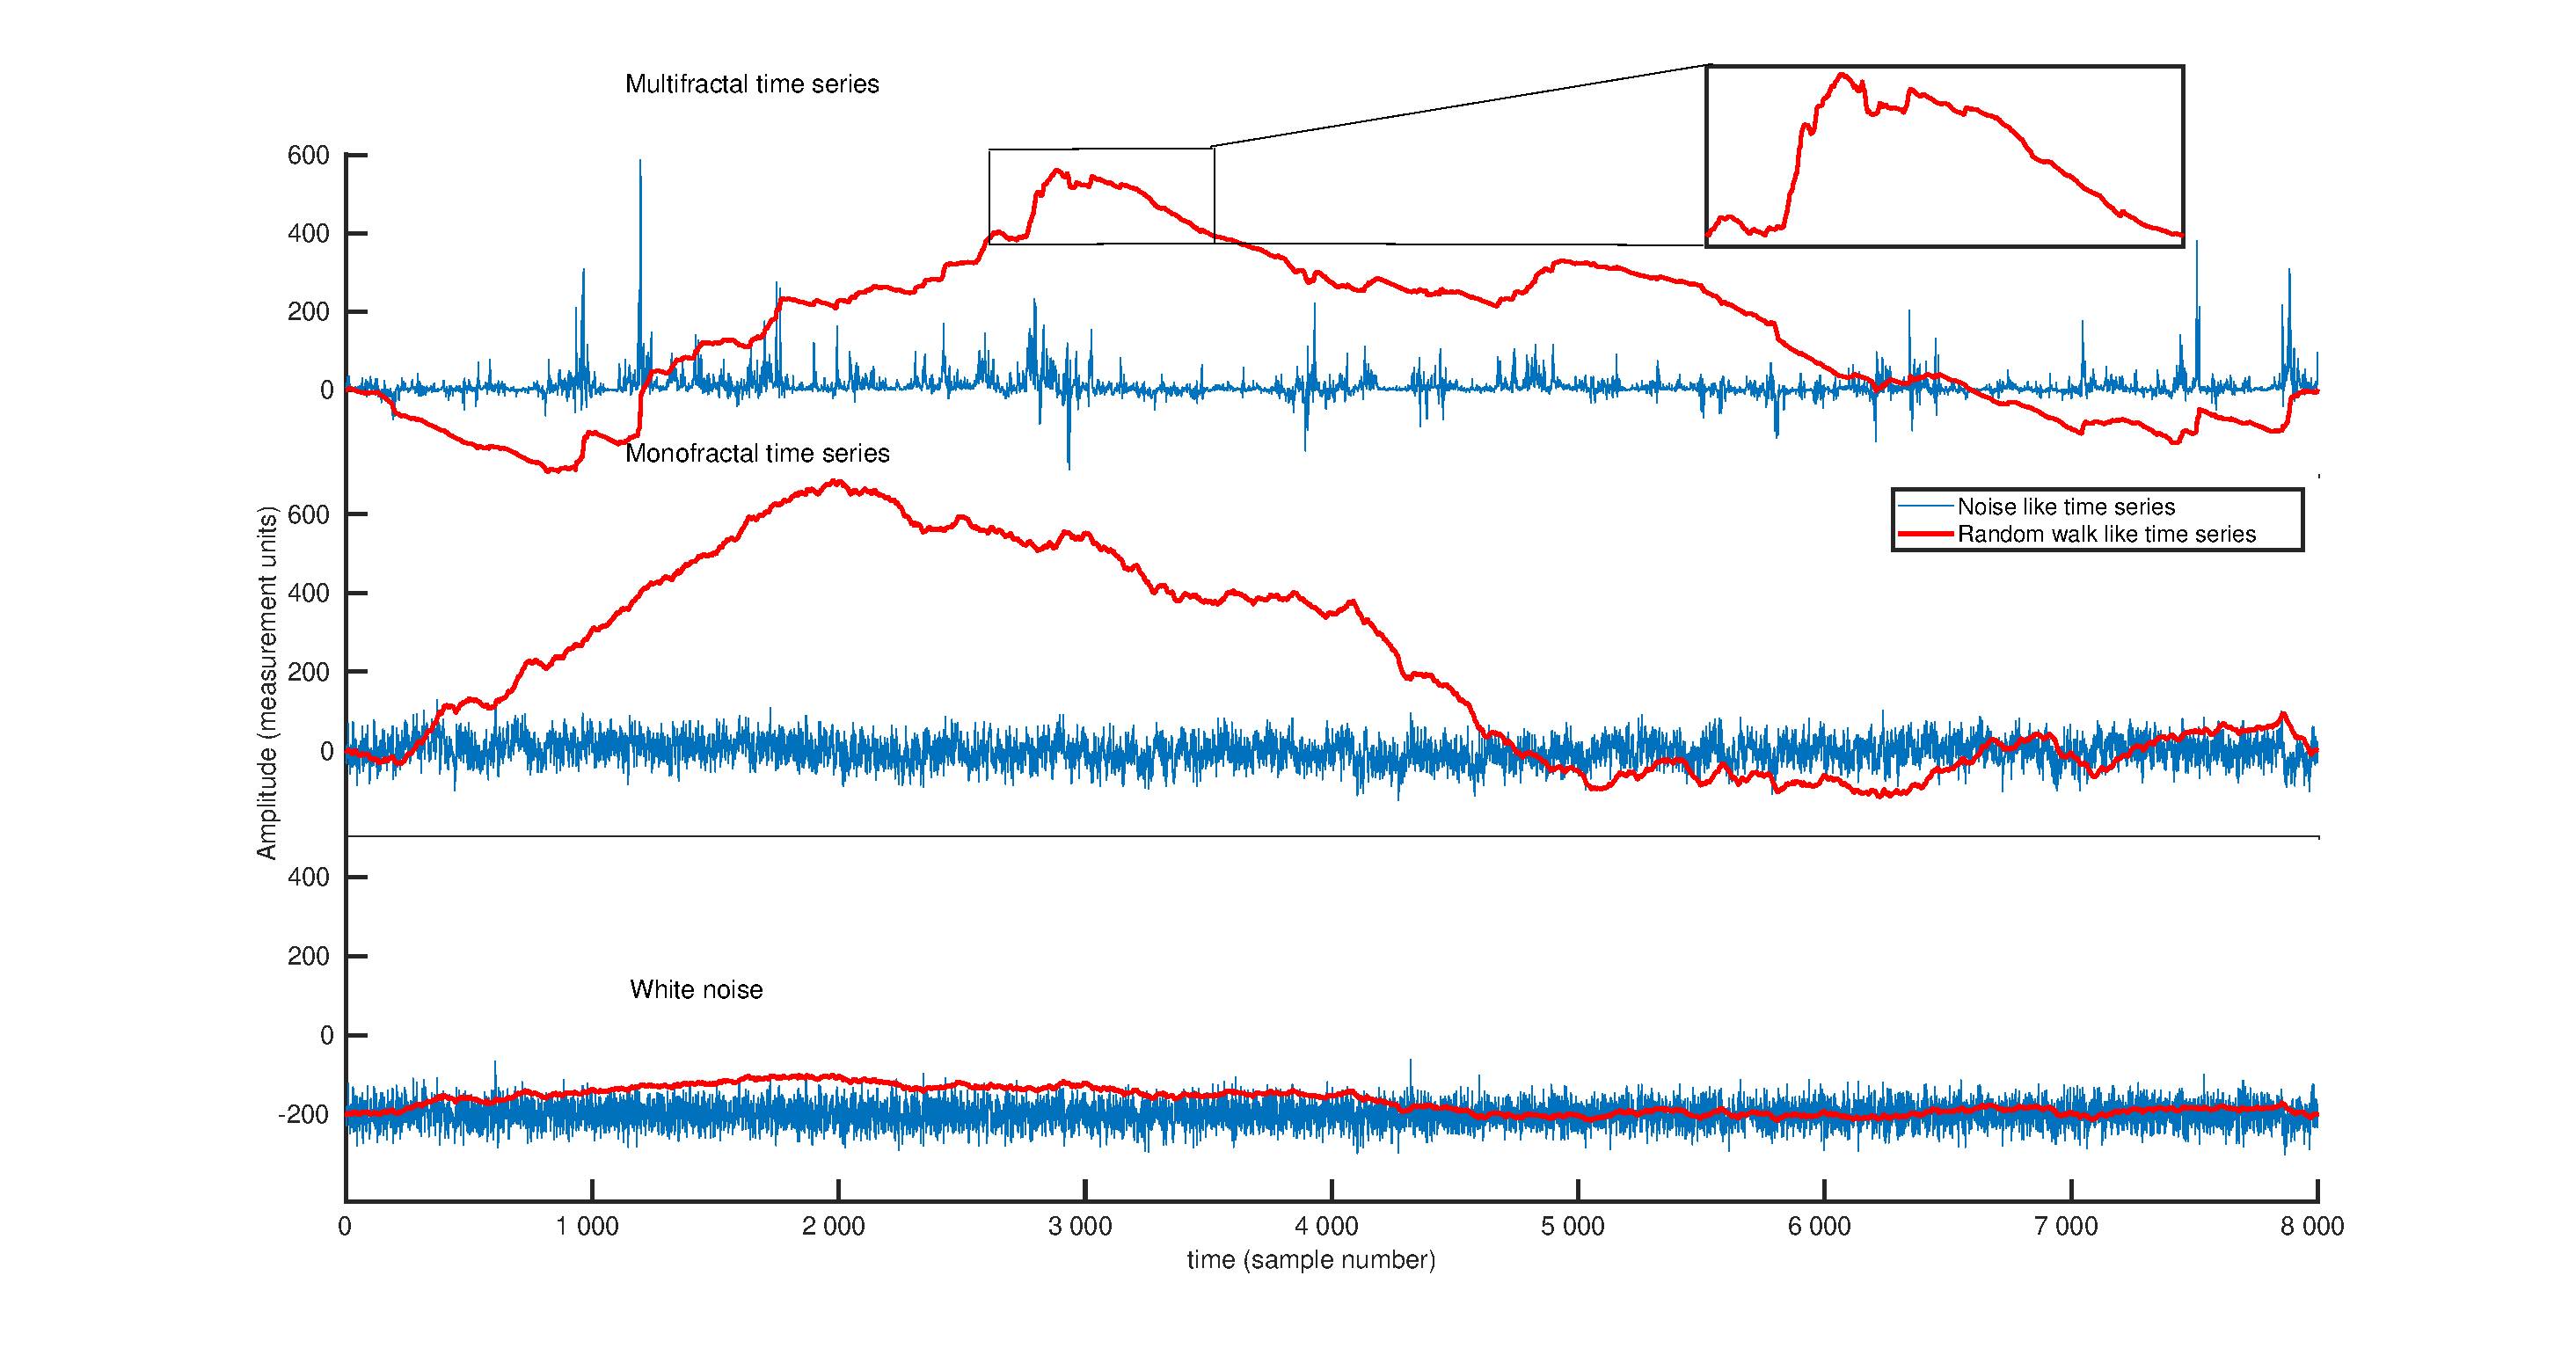
\includegraphics[width=12cm]{fig1.eps}
		\caption{\textit{Random walks} e fractalidade.}
	\end{figure}
	Observa-se com elevado detalhe como h\'a de fato fractalidade nas \textit{random walks} geradas
	a partir das s\'eries factrais, o que \'e bem interessante, e bem diferente quando comparado
	com a \textit{random walk} gerada pelo ru\'ido branco, a qual possui at\'e mesmo
	quase que uma periodicidade de amplitude muito baixa.
	\section{Figura 2}
	Realizando os comandos indicados no artigo em \textit{Matlab}, que calculam a ra\'iz da
	m\'edia das s\'eries temporais originais com o aux\'ilio da sintaxe do \textit{Matlab}:
	\begin{figure}[H]
		\centering
		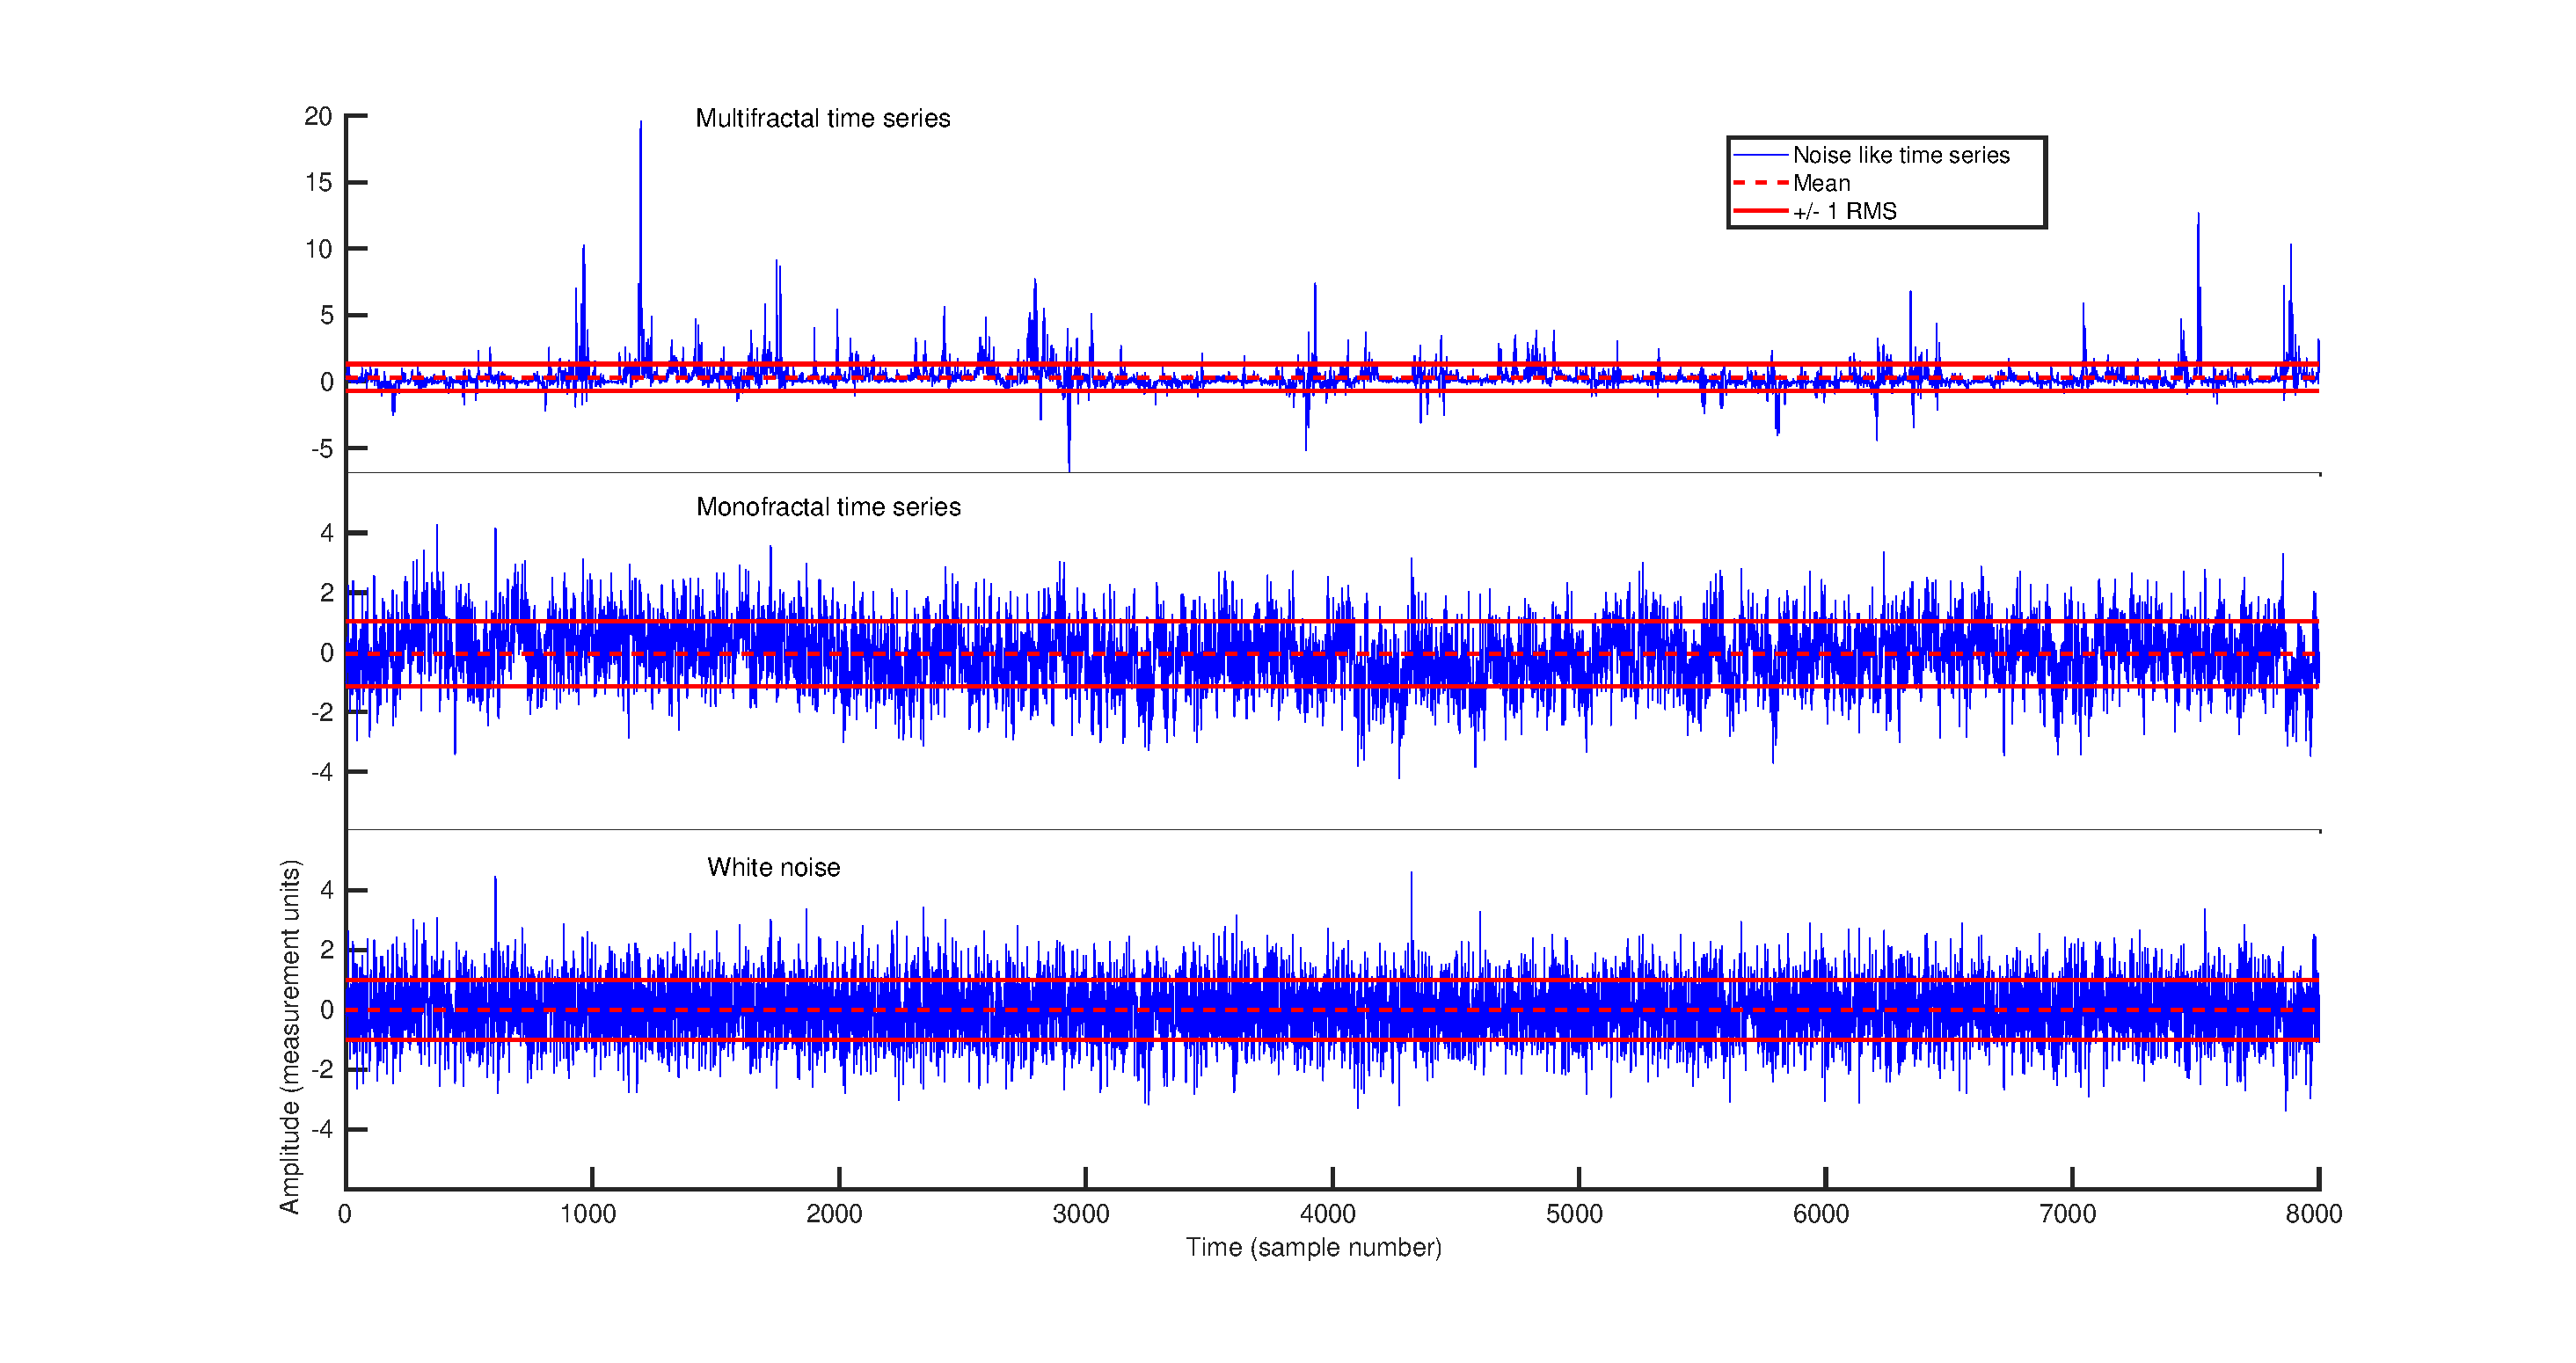
\includegraphics[width=12cm]{fig2.eps}
		\caption{\textit{Root mean square} global.}
	\end{figure}
	Confirma-se como, apesar de n\~ao parecer em virtude da mudan\c{c}a da escala entre figuras,
	todas as s\'eries possuem m\'edia 0 e \textit{RMS} 1, incapazes de descrever bem as s\'eries.
	\section{Figura 3}
	Realizando os comandos indicados no artigo em \textit{Matlab}, que dividem a s\'erie temporal
	em diversos segmentos, interpola cada um e a partir da interpola\c{c}\~ao calculam a
	\textit{root mean square} do segmento:
	\begin{figure}[H]
		\centering
		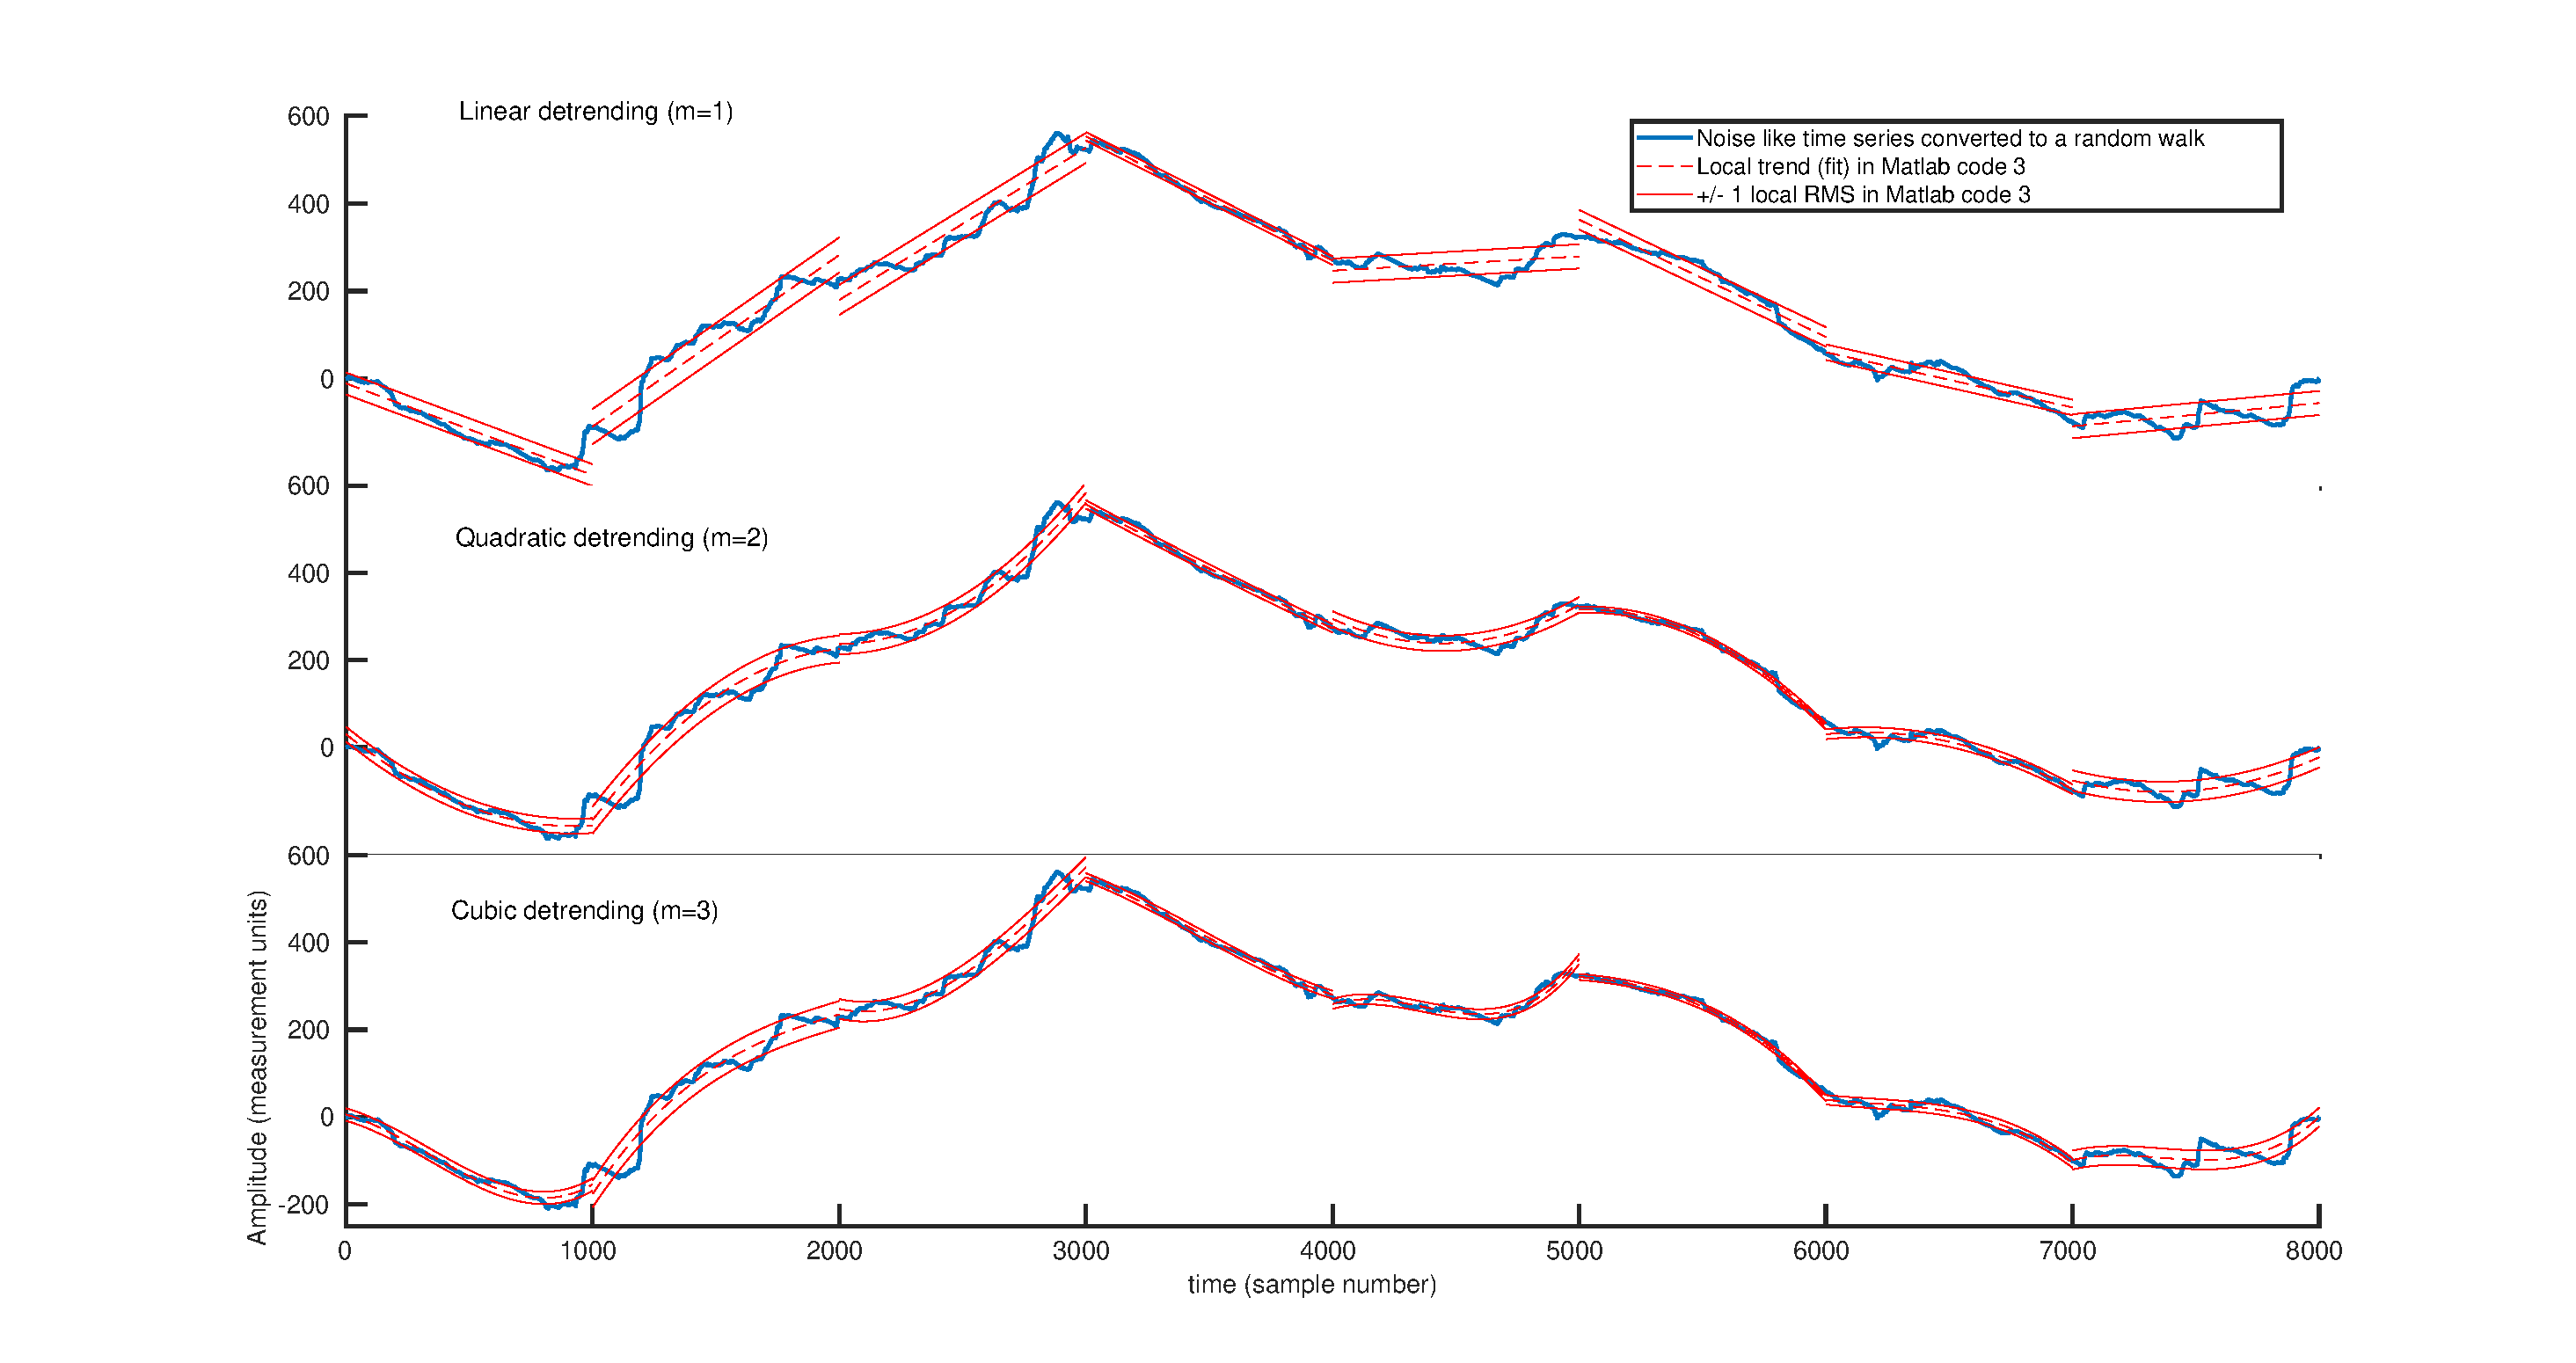
\includegraphics[width=12cm]{fig3.eps}
		\caption{\textit{Root mean square} local.}
	\end{figure}
	O que se pode observar diretamente \'e como de fato considerar localmente acumula muito
	mais informa\c{c}\~ao do que quando se considera globalmente, o que faz sentido. Tamb\'em
	se pode perceber o por que de uma interpola\c{c}\~ao de ordem 3 ser mais interessante; se
	o gr\'afico com m = 1 for analisado, verifica-se que a reta falha em capturar tend\^encia
	local pois n\~ao consegue acompanhar a curva, efeito que \'e mitigado quando se aumenta
	a ordem, tanto que se observa uma boa diferen\c{c}\~ao no valor do \textit{root mean
	square} conforme se aumenta a ordem da interpola\c{c}\~ao, em alguns dos segmentos.
	\section{Figura 4}
	Realizando os comandos indicados no artigo em \textit{Matlab}, que realizam o mesmo procedimento
	feito na figura 3, por\'em em um la\c{c}o que varia o n\'umero de segmentos, e no final
	calculando o \textit{root mean square} dos \textit{root mean squares} de cada segmento:
	\begin{figure}[H]
		\centering
		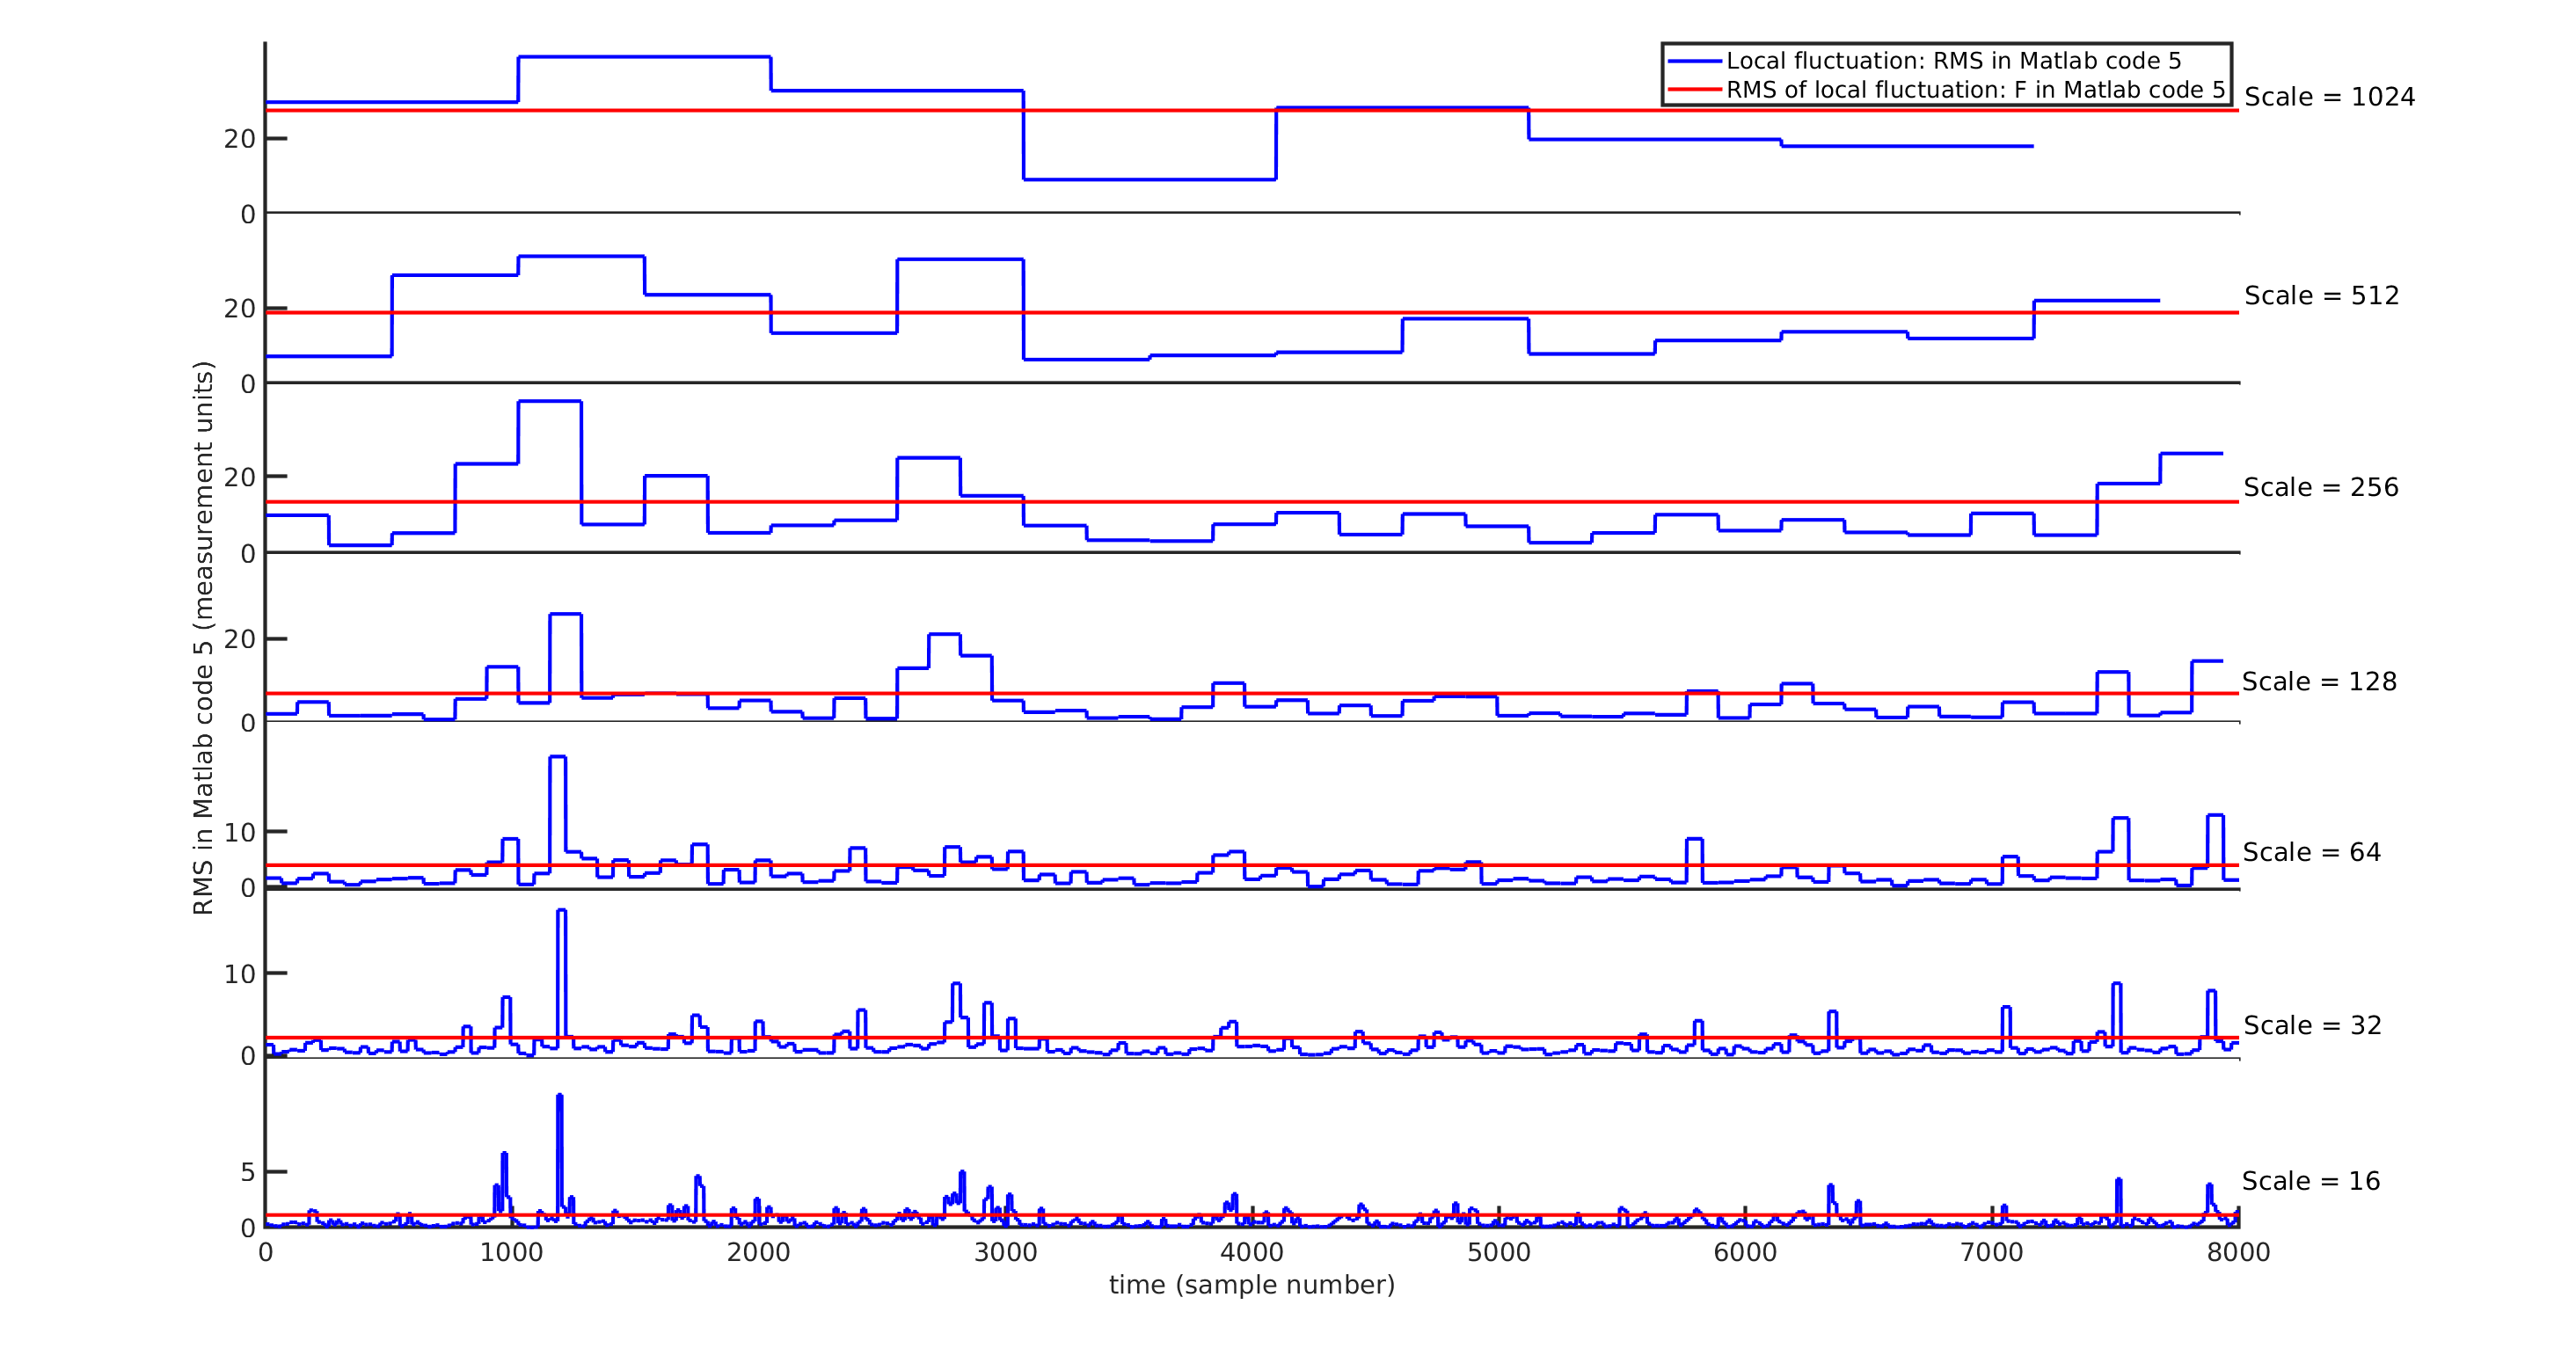
\includegraphics[width=12cm]{fig4.eps}
		\caption{\textit{Detrended fluctuation analysis}.}
	\end{figure}
	O que \'e coerente com o previsto, levando-se em considera\c{c}\~ao que a s\'erie
	temporal sendo estudada nesta figura \'e a multifractal: ela possui flutua\c{c}\~oes
	que mudam mais lentamente, as quais s\~ao capturadas por esse procedimento feito com
	segmentos maiores, o que \'e algo que faz sentido. Caso fossem utilizados segmentos muito
	pequenos, todos eles iriam ter \textit{RMS} nulos pois localmente n\~ao h\'a muita
	varia\c{c}\~ao, dado que as flutua\c{c}\~oes s\~ao lentas.
	\section{Figura 5}
	Realizando os comandos indicados no artigo em \textit{Matlab}, que utilizam a m\'etrica
	definida na Figura 4 e com os dados dela realizam regress\~ao linear em espa\c{c}o log,
	para ent\~ao encontrar o expoente de \textit{Hurst}:
	\begin{figure}[H]
		\centering
		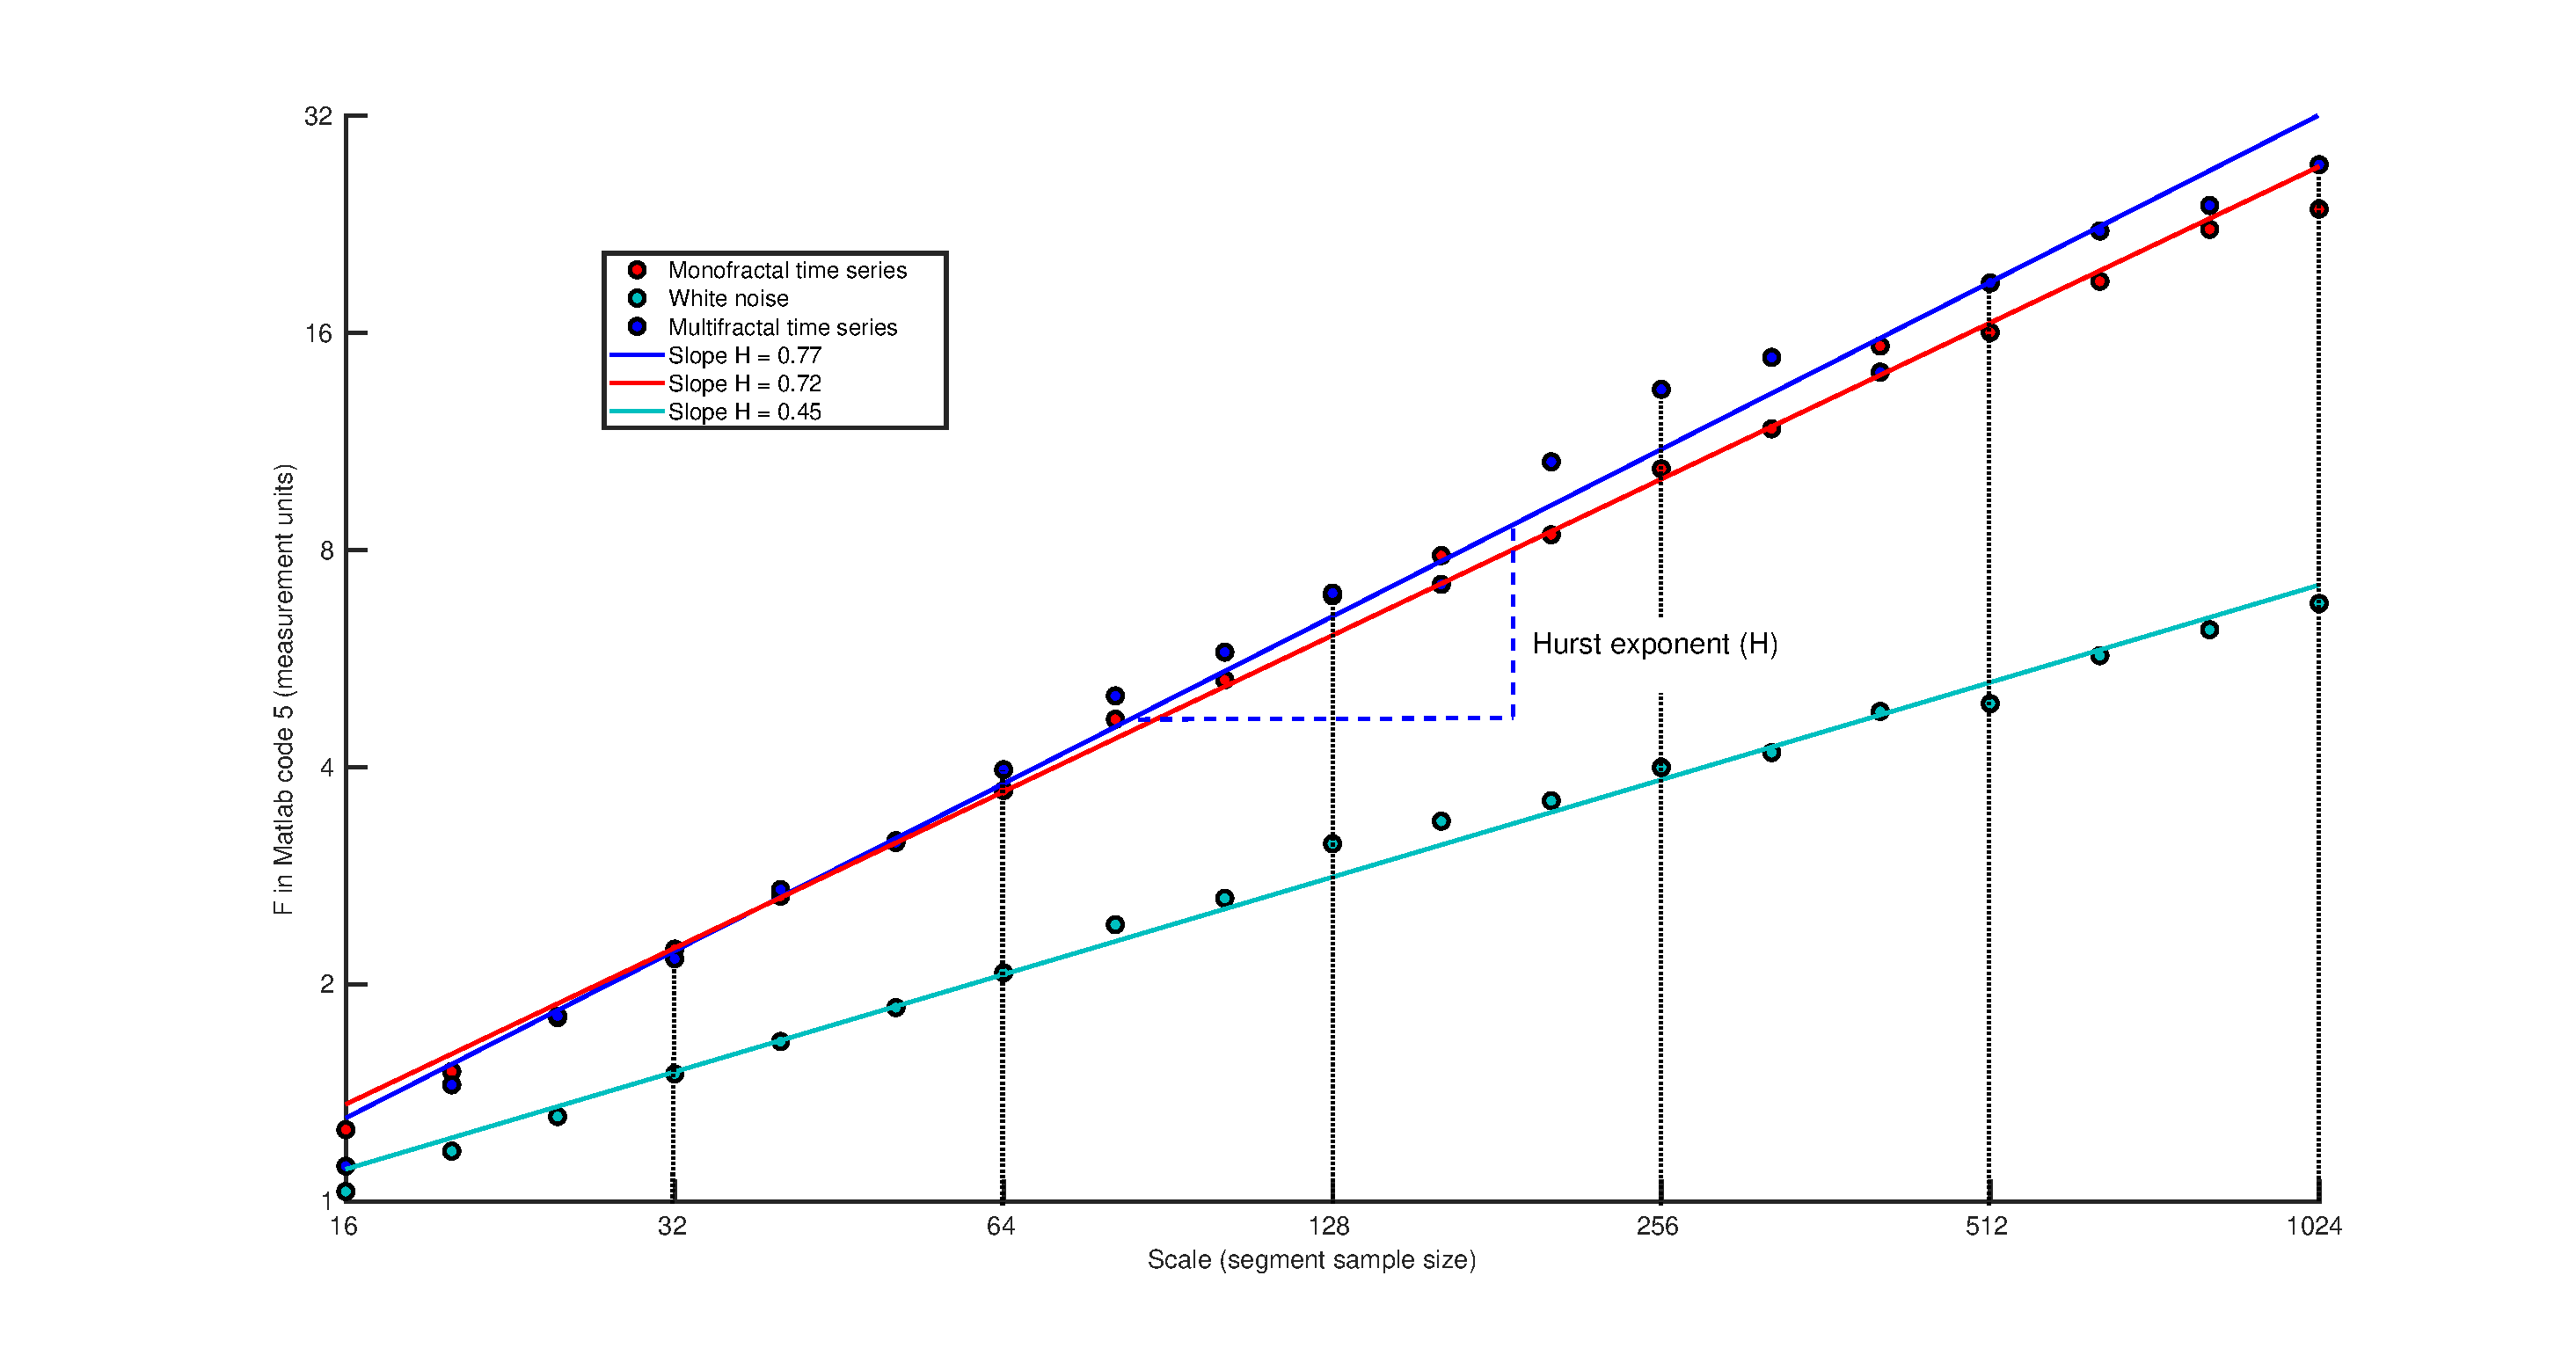
\includegraphics[width=12cm]{fig5.eps}
		\caption{Expoente de \textit{Hurst}.}
	\end{figure}
	Onde se pode ver como o expoente de \textit{Hurst}, a inclina\c{c}\~ao da reta, realmente
	define e diferencia entre cada s\'erie temporal, pois ele define a varia\c{c}\~ao
	da \textit{Detrended Fluctuation Analysis}, a qual, por ser um ind\'icio de flutua\c{c}\~oes
	lentas, \'e capaz de distinguir entre ru\'ido branco e outras s\'eries que possuem
	mais previsibilidade.
\end{document}
